% --- CHUNK_METADATA_START ---
% needs_review: True
% src_checksum: 5da0735687c2aea3697e5e896ffcb2de79d53828c4ce70778e3f5615aecdb14a
% --- CHUNK_METADATA_END ---
\chapter{Евклідові простори}% --- CHUNK_METADATA_START ---
% needs_review: True
% src_checksum: 09c6effe383b397c2e287b2302b5c82f4782172b70cdf3be336a68a99ec35441
% --- CHUNK_METADATA_END ---
«Класична» лінійна алгебра розглядає векторні простори, де мова йде лише про лінійні комбінації, підпростори, бази, матриці тощо. У певний момент цього стає недостатньо. Щоб мати можливість досліджувати сильніші, складніші та корисніші поняття, нам потрібно буде обчислювати довжину вектора, кути між двома векторами, відносне розташування між векторами тощо. Щоб мати можливість вивчати ці концепції, ми вводимо поняття скалярного добутку (білінійної форми) і, отже, векторних просторів, забезпечених цим добутком.

Цей розділ присвячений вивченню двох основних понять:% --- CHUNK_METADATA_START ---
% needs_review: True
% src_checksum: 70055e76d35e68266dcc2b09983fa30f0cc425313d489a398c66762a9624032b
% --- CHUNK_METADATA_END ---
\begin{itemize}
    \item скалярні добутки
    \item евклідові простори
\end{itemize}% --- CHUNK_METADATA_START ---
% needs_review: True
% src_checksum: 479ce8267a8dc66449e53b838492edeab11f9f116eed87da087547c1cd388ae6
% --- CHUNK_METADATA_END ---
\section{Вступ}% --- CHUNK_METADATA_START ---
% needs_review: True
% src_checksum: 0ac44e2012e6f37806b8ec7c72ad867302be795f6c99ca78cd8ba87ccba55dd5
% --- CHUNK_METADATA_END ---
Векторні простори, які розглядаються в цьому розділі, є дійсними. Припускається, що $E$ є $\R$-векторним простором.

Скалярний добуток:% --- CHUNK_METADATA_START ---
% needs_review: True
% src_checksum: aac3ae1bec48ecd43cdb867de27dbe9d4e32a291690935f3e07ad94ea30b3963
% --- CHUNK_METADATA_END ---
\begin{definition}
    Білінійна форма на $E$ — це відображення  
    \begin{align*}
        B: E \times E &\longrightarrow \R \\
        (u, v) &\longmapsto B((u, v))
    \end{align*}
    що задовольняє наступні умови $\forall u, v, w \in E$ $\forall \lambda \in \R$:
    \begin{enumerate}
        \item $B(u + \lambda v, w) = B(u, w) + \lambda B(v, w)$
        \item  $B(u, v + \lambda w) = B(u, v) + \lambda B(v, w)$
    \end{enumerate}
    B називається 
    \begin{enumerate}
        \item симетрична якщо $B(u, v) = B(v, u)$  $\forall u, v \in E$
        \item позитивна якщо $B(., u) \ge 0 \, \forall u \in E$
        \item визначена якщо $B(u, u) = 0 \iff u = 0$
    \end{enumerate}
\end{definition}% --- CHUNK_METADATA_START ---
% needs_review: True
% src_checksum: b3e3014d86bf527aed2249534faff461531a00e3c7469faa8feaef31f7788090
% --- CHUNK_METADATA_END ---
\begin{notation}
   Скалярний добуток позначається: $<u, v>$ 
\end{notation}% --- CHUNK_METADATA_START ---
% needs_review: True
% src_checksum: 8c68c516bc5901f21ff7541f291db7303a684176baa8fee049e9397452534c86
% --- CHUNK_METADATA_END ---
\begin{eg}.
   \begin{enumerate}
       \item $E = \R^n$,  $X = (x_1, \ldots, x_n), Y = (y_1, \ldots, y_n) \in E$\\
           \[
               <X, Y> := \sum_{n=1}^{n} x_iy_i
           \] 
           Його називають "канонічним скалярним добутком" (або звичайним)
        \item $E = \R^2$ і  $<X, Y> = 2x_1y_1 + x_2y_2$
        \item $E = \mathcal{C}^0([-1, 1], \R) \ni f, g$ (простір неперервних функцій)
            \[
                <f, g> := \int_{-1}^{1} f(t) \cdot g(t) \: d{t} 
            \] 
        \item $E = \mathcal{M}_n(\R) \ni A, B$
             \[
            <A, B> := Tr(A^tB)
            \] 
   \end{enumerate} 
\end{eg}% --- CHUNK_METADATA_START ---
% needs_review: True
% src_checksum: 3754243cd92b07a4e8a3690f08a016f59688f2b965a017a38bca50239762e19f
% --- CHUNK_METADATA_END ---
\begin{prop}
    Ненульовий векторний простір має нескінченну кількість різних скалярних добутків.   
\end{prop}% --- CHUNK_METADATA_START ---
% needs_review: True
% src_checksum: 73752ce65fbe2fdff7cab331cd5cc247e172ed8b55063a0cfebe8d6a4a21be40
% --- CHUNK_METADATA_END ---
\begin{definition}
    Евклідовий простір — це пара $(E, < . >)$, де $E$ є $\R$-векторним простором \underline{скінченновимірним} та $< . >$ є скалярним добутком на $E$.
\end{definition}% --- CHUNK_METADATA_START ---
% needs_review: True
% src_checksum: de6e7256acedf77ba6b59dd8c8638e3b17598fcb2783a559a6ba2e747ecc603d
% --- CHUNK_METADATA_END ---
\begin{property} Нехай $(E, < . >)$ евклідів простір. Покладемо:
    \[
    \|X\| := \sqrt{<X,X>} \qquad X \in E 
    \] 
    норма (або довжина) $X$. (Вона добре визначена, оскільки $<., .>$ завжди позитивний)
\end{property}% --- CHUNK_METADATA_START ---
% needs_review: True
% src_checksum: a0c34c74b776c4b2712e0bc68ea2baf5a169429392c9041fa9951ee767e094fd
% --- CHUNK_METADATA_END ---
\begin{property}
   Нехай $X, Y \in E$, тоді:
   \[
       \|X + Y\|^2 = \|X\|^2 + 2\scalair{X, Y} + \|Y\|^2
   \] 
\end{property}% --- CHUNK_METADATA_START ---
% needs_review: True
% src_checksum: 8432f24eca144a9f41a6cbb5161d6ea135f840aad65be511c92557c145409cf5
% --- CHUNK_METADATA_END ---
\begin{proof}
   \begin{align*}
       \|X + Y\|^2 = \sqrt{\scalair{X + Y, X + Y}}^2 &= \scalair{X + Y, X + Y} \\ 
                                                     &= \scalair{X, X + Y} + \scalair{Y, X + Y}  \\
                                                     &= \scalair{X, X} + \scalair{X, Y} + \scalair{Y, X} + \scalair{Y, Y}\\
                                                     &= \|X\|^2 + 2\scalair{X, Y} + \|Y\|
   \end{align*} 
\end{proof}% --- CHUNK_METADATA_START ---
% needs_review: True
% src_checksum: 01d462ad6bb3b1ce2908c760049b50ee548204ecba31f845da8c1db0f8bf13f6
% --- CHUNK_METADATA_END ---
\begin{lemma}\label{lemma:inegalite-cauchy-schwarz} нерівність Коші-Шварца
   Маємо
   \[
   |<u, v>| \le \|u\| \cdot \|v\| \qquad \forall u, v \in E
   \] 
   з рівністю тоді і тільки тоді, якщо $u$ та $v$ колінеарні, тобто $\exists \, t \in R$ такий, що $u = tv$ або $v = tu$
\end{lemma}% --- CHUNK_METADATA_START ---
% needs_review: True
% src_checksum: dd7937806464a5e6da7e6b458df5a7ae1a082e9a65aec713595521a1e6323273
% --- CHUNK_METADATA_END ---
\begin{explanation}
   Якщо $v = 0$, зрозуміло\\
   Якщо $v \neq 0$ розглянемо $\forall t \in \R$
   \begin{align*}
       \|u + tv\|^2 &= <u + tv, u + tv>\\ 
                    &= <u, u + tv> + t<v, u + tv>\\
                    &= <u, u> + t<u, v> + t<v, u> + t^2<v, v>\\
                    &= \|u\|^2 + 2t<u, v> + t^2 \|v\|^2 = f(t)
   \end{align*}
   \begin{center}
       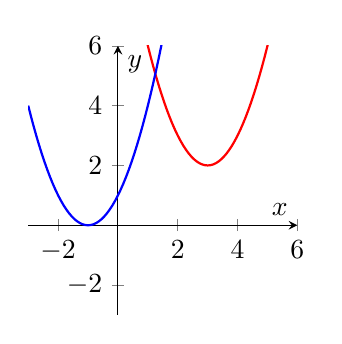
\begin{tikzpicture}
           \begin{axis}[
               axis lines = center,
               xlabel = $x$,
               ylabel = $y$,
               samples = 100,
               domain = -3:6,
               xmin = -3, xmax = 6,
               ymin = -3, ymax = 6,
               width=5cm,
               height=5cm
               ]
               \addplot[red, thick] {(x - 3)^2 + 2};
               \addplot[blue, thick] {(x + 1)^2};
           \end{axis}
       \end{tikzpicture}
   \end{center}
Випадок 1: $f(t)$ не має різних коренів
\begin{align*}
    &\Delta = 4<u, v>^2 = 4\|u\|^2\|v\|^2 \le 0\\
    \implies & <u, v>^2 \le \|u\|^2 \cdot \|v\|^2\\
    \implies & |<u, v>| \le \|u\|\|v\|
\end{align*}
Випадок 2: $f(t)$ має лише один корінь:
\begin{align*}
    &\Delta = 0\\
    \implies & \exists t \in \R \text{ така що } \|u + tv\|^2 = 0\\
    \implies &u + tv = 0 \implies u = -tv
\end{align*}
\end{explanation}% --- CHUNK_METADATA_START ---
% needs_review: True
% src_checksum: c1714456eb2dec6573390652b4931da225ab71012c26330b844da6910872d60d
% --- CHUNK_METADATA_END ---
Наступне визначення буде вивчено в курсі аналізу:% --- CHUNK_METADATA_START ---
% needs_review: True
% src_checksum: 7f4d91e24d8e87eb9d751db268d06f36046760b562f9679cbc4ec4ec849c4e91
% --- CHUNK_METADATA_END ---
\begin{definition}
    Кажуть, що $N: E \to \R_+$ є нормою, якщо:
    \begin{enumerate}
        \item $N(\lambda u) = |\lambda| \cdot N(u)$ \quad  $\forall \lambda \in \R, \forall u \in E$
        \item $N(u) = 0 \implies u = 0$
        \item $N(u + v) \le N(u) + N(v)$ \quad $\forall u, v \in E$
    \end{enumerate}
\end{definition}% --- CHUNK_METADATA_START ---
% needs_review: True
% src_checksum: 29fe003cc6ce4d1aea6b0410774a5d08729125a2118436a2ce7784a58c116681
% --- CHUNK_METADATA_END ---
\begin{lemma}
   Відображення
   \[
   \sqrt{<.,.>} = \| . \|: E \to \R_+ 
   \] 
   називається евклідовою нормою.
\end{lemma}% --- CHUNK_METADATA_START ---
% needs_review: True
% src_checksum: 7c736f0253c57b9007eb5f8c29d4e29b3a3e6059a266b244847745b6ff0c0277
% --- CHUNK_METADATA_END ---
\begin{explanation}
    1), 2) зроблено\\
    \begin{itemize}
        \item[3)] $\| u + v \|^2 = \|u\|^2 + 2<u,v> + \|v\|^2 \le \|u\|^2 + 2\|u\|\|v\| + \|v\|^2 = (\|u\| + \|v\|)^2$
            \[
            \implies \|u + v\|^2 \le \|u\|^2 + \|v\|^2
            \] 
    \end{itemize}
\end{explanation}% --- CHUNK_METADATA_START ---
% needs_review: True
% src_checksum: 6fc2f21b40ab21daed7de5d63fc64583726c71d583db47bd8bf31d39bc96c70e
% --- CHUNK_METADATA_END ---
\begin{prop}
   Маємо наступні тотожності $\forall u, v \in E$ 
   \begin{enumerate}
       \item Тотожність паралелограма:
           \[
           \|u + v\|^2 + \|u - v\|^2 = 2(\|u^2\| + \|v\|^2)
           \] 
       \item Тотожність поляризації:
           \[
               \scalair{u, v} = \frac{1}{4}(\|u + v\|^2 - \|u - v\|^2)
           \] 
   \end{enumerate}
\end{prop}% --- CHUNK_METADATA_START ---
% needs_review: True
% src_checksum: 8ea48ceb96f53479a13cb0809bb9b4c21c511cb1436fe021b40a9523876d5a28
% --- CHUNK_METADATA_END ---
\begin{explanation}.
   \begin{enumerate}
       \item 
           \begin{align*}
               \|u + v\|^2 &= \scalair{u + v, u + v}\\
                           &= \|u\|^2 + 2\scalair{u,v} + \|v\|^2
           \end{align*}
       \item $\|u - v\|^2 = \|u\|^2 - 2\scalair{u, v} + \|v\|^2$
   \end{enumerate} 
   Маємо:
   \begin{itemize}
       \item 
           $(1) + (2)$:  $\|u + v\|^2 + \|u - v\|^2 = 2 (\|u\|^2 + \|v\|^2)$
       \item $(1) - (2)$:  $\|u + v\|^2 - \|u - v\|^2 = 4\scalair{u, v}$ 
   \end{itemize}
\end{explanation}% --- CHUNK_METADATA_START ---
% needs_review: True
% src_checksum: c705ccdbbe83531645858a091730563d185c1d4357934fea51fc437d8c8d25c7
% --- CHUNK_METADATA_END ---
\section{Ортогональність}% --- CHUNK_METADATA_START ---
% needs_review: True
% src_checksum: 3b7793f1f64934c9b08010a74f388a75b5aebd58d5c0eabfab6bb9d63a13877c
% --- CHUNK_METADATA_END ---
Нехай $E$ буде $\R$-векторним простором і $\scalair{ , }$ скалярним добутком на $E$.% --- CHUNK_METADATA_START ---
% needs_review: True
% src_checksum: a50d257209420676b32029c180974a5ba8ce99821cf6bb087f70ea743ed18003
% --- CHUNK_METADATA_END ---
\begin{definition}\label{def:orthogonal}
     $u, v \in E$ називаються \underline{ортогональними} якщо $<u, v> = 0$. Позначають $u \perp v$
      \begin{itemize}
         \item Дві підмножини $A, B$ з $E$ є ортогональними якщо:
              \[
             \forall u \in A, \forall v \in B, \quad <u, v> = 0
             \] 
         \item Якщо $A \subseteq E$ називають \textbf{ортогональним до $A$}, що позначається $A^{\perp}$ множину
              \[
                  A^{\perp} = \{ u \in E \mid <u, v> = 0 \quad \forall v \in A \}
             \] 
             Також відомий як \textbf{ортогональне доповнення $A$}
         \item Сімейство $(v_1, \ldots, v_n)$ векторів з $E$ називається ортогональним, якщо $\forall i \neq j, v_i \perp v_j$. Воно називається ортонормованим, якщо воно ортогональне, і крім того $\|v_i\| = 1 \quad \forall i \in \{ 1, \ldots, n \}$
     \end{itemize}
\end{definition}% --- CHUNK_METADATA_START ---
% needs_review: True
% src_checksum: 0fea0c9eedad08e574166dbfecd45aa77a49a34b6c1afc0c8c3ca35b679e2395
% --- CHUNK_METADATA_END ---
\begin{eg}
   $E = \R^n$,  $< , >$ канонічний скалярний добуток 
   \[
       v_i = (0, \ldots, 0, \underbrace{1}_{i}, 0, \ldots, 0)
   \] 
   \[
   <v_i, v_j> = \begin{cases}
       1 \text{ якщо } i = j\\  
       0 \text{ якщо } i \neq  j
   \end{cases}
   \] 
   $(v_1, \ldots, v_n)$ є канонічним базисом
\end{eg}% --- CHUNK_METADATA_START ---
% needs_review: True
% src_checksum: 6fe38b98e0c58272e2277c935867cc0f2da465ae23e70ab50ffbf4a07fbe2003
% --- CHUNK_METADATA_END ---
\begin{prop}
    \begin{enumerate}
        \item 
            Якщо $A \subseteq E$ тоді $A^{\perp}$ є векторним підпростором $E$ 
        \item Якщо $A \subseteq B$ тоді $B^{\perp} \subseteq A^{\perp}$
        \item $A^{\perp} = Vect(A)^{\perp}$
        \item $A \subset (A^{\perp})^{\perp}$ 
    \end{enumerate}
\end{prop}% --- CHUNK_METADATA_START ---
% needs_review: True
% src_checksum: 19b7087b6a48384d722d6b841661a817b54245a8f5f18649f66ec1bddb8ac4ac
% --- CHUNK_METADATA_END ---
\begin{explanation}
   Вправа 
\end{explanation}% --- CHUNK_METADATA_START ---
% needs_review: True
% src_checksum: 0c811ad2e1c9baccb837657ac7fe9c9e79bf8a8869817013fbeebbc1fee459ad
% --- CHUNK_METADATA_END ---
\begin{eg}
   \begin{enumerate}
       \item $E = \mathcal{C}^0([-1, 1], \R)$
            \[
                <f, g> := \int_{-1}^{1} f(t) \cdot g(t) \: d{t} 
            \] 
            \begin{center}
       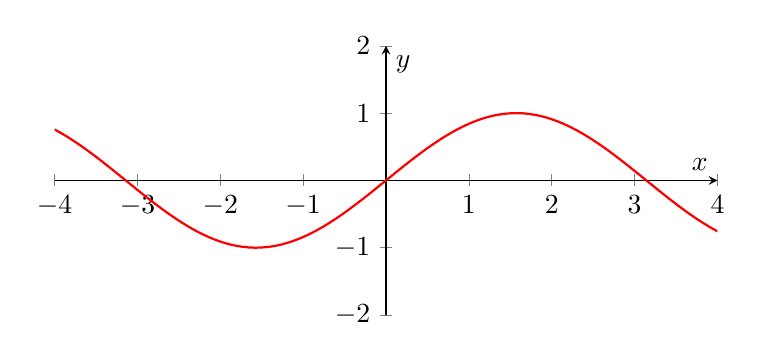
\begin{tikzpicture}
           \begin{axis}[
               axis lines = center,
               xlabel = $x$,
               ylabel = $y$,
               samples = 100,
               domain = -4:4,
               xmin = -4, xmax = 4,
               ymin = -2, ymax = 2,
               width=10cm,
               height=5cm
               ]
               \addplot[red, thick] {sin(deg(x))};
           \end{axis}
       \end{tikzpicture}
   \end{center}
   Тоді, $f(t) = \cos(t)$, $g(t) = \sin(t)$ ортогональні: $2\cos(t)\sin(t) = \sin(2t)$
   \[
       \int_{-1}^{1} \cos(t)\sin(t)\:d{t} = \frac{1}{2}\int_{-1}^{1} \sin(2t) \: d{t} = 0  
   \] 
   \end{enumerate} 
\end{eg}% --- CHUNK_METADATA_START ---
% needs_review: True
% src_checksum: 34a1b6efd8afd5a191fedcc4063c7162e4ff251b3b80e839ad5d5aa5c887835f
% --- CHUNK_METADATA_END ---
\begin{definition}
    Якщо $E$ є евклідовим простором, ми називаємо "дуал $E$" множину
    \[
        L(E, \R) = \{ f: E \to \R \mid f \text{ є лінійною}\}
    \] 
    Його позначають $E^*$. Елемент $f \in E^*$ називається лінійною формою.
\end{definition}% --- CHUNK_METADATA_START ---
% needs_review: True
% src_checksum: 3b0fe845bcfce365ebe09bee7ac9bde0d0486f12b24754d48e80e6331fd867ae
% --- CHUNK_METADATA_END ---
Нагадаємо:% --- CHUNK_METADATA_START ---
% needs_review: True
% src_checksum: c62046bf44d7a01ed59a1a4b7bea4075b61a00b15df8ed0bc5edfae3be41e91d
% --- CHUNK_METADATA_END ---
\begin{prop}
    Якщо $F, F'$ — два скінченновимірні в.п., то $dim(L(F, F')) = dim(F)\cdot dim(F')$\\
    Зокрема, $dim(F^*) = dim(F)$. Справді, якщо $n = (e_1, \ldots, e_p)$ є базисом $F$ є $n' = (e'_1, \ldots, e'_q)$ є базисом $F'$, то відображення
    \begin{align*}
        : L(F, F') &\longrightarrow Mat_{f\times p}(\R) \\
        f &\longmapsto (f) = Mat_{n,n'}(f)
    .\end{align*}
    є ізоморфізмом. Отже $dim(F, F) = qp$
\end{prop}% --- CHUNK_METADATA_START ---
% needs_review: True
% src_checksum: c9aa8b287720d3caad43357c6f50e57667cb4596ca051151224ebd08f7781253
% --- CHUNK_METADATA_END ---
\begin{theorem}
    Теорема про ранг: Якщо $F$ є скінченновимірним векторним простором і $f: F \to F'$ лінійне, тоді $dim(F) = dim(Ker(f)) + dim(Im(f))$
\end{theorem}% --- CHUNK_METADATA_START ---
% needs_review: True
% src_checksum: d2a5584e9f9f2893dffad3bfa59128e0eff437ca2b8cc8fdfdca03e8312c5f4a
% --- CHUNK_METADATA_END ---
\begin{prop}
    Якщо $F, F'$ є два векторні простори \underline{скінченновимірні} такі що $dim(F) = dim(F')$ і  $f: F \to F'$ лінійне, тоді $f$ є ізоморфізмом $\iff Ker(f) = {0}$
\end{prop}% --- CHUNK_METADATA_START ---
% needs_review: True
% src_checksum: 6c10e113159dc42fee26f775e32f5b658f01d15a5a580ec4fb86fb5c44d8a610
% --- CHUNK_METADATA_END ---
\begin{explanation}
   Нагадаємо, що якщо $G, G'$ є скінченновимірними підпросторами в тому ж векторному просторі, тоді:
   \[
   G = G' \iff G \subseteq G' \text{ і } dim(G) = dim(G')
   \] 
   $\implies$) $f$ ін'єктивне $\implies$ $Ker(f) = {0}\\$
   $\impliedby$) Нехай $Ker(f) = {0}$.\\
   Тоді, обов'язково $dim(Ker(f)) = 0$ і за теоремою про ранг ми маємо $dim(F) = dim(Im(f))$, тому $Im(f) = F'$
\end{explanation}% --- CHUNK_METADATA_START ---
% needs_review: True
% src_checksum: 96310fb223d39512a621685fe14d4231b8b736cf346ef901b9446c1f0f46329a
% --- CHUNK_METADATA_END ---
\begin{lemma} лема Ріса:\\
    Нехай $(E, \scalair{.,.})$ скінченновимірний евклідовий простір і $f \in E^*$. Тоді, $\exists! u \in E$ такий що $f(x) = \scalair{u, x} \quad \forall x \in E$. Лінійна форма $f$ задається скалярним добутком з вектором. 
\end{lemma}% --- CHUNK_METADATA_START ---
% needs_review: True
% src_checksum: db83365bab1f1a066c9d4aceecc2aaa09b915c739ca3c1af5b5b251e538fbf9e
% --- CHUNK_METADATA_END ---
\begin{notation}
   Для будь-якого $v \in E$ позначаємо через $f_v$ відображення:
   \begin{align*}
       f_v: E &\longrightarrow \R \\
       x &\longmapsto f_v(x) = <v, x>
   .\end{align*}
   $f_v$ є лінійним $\forall v \in E$ тобто $E^*$
\end{notation}% --- CHUNK_METADATA_START ---
% needs_review: True
% src_checksum: b785e304a80823e3776a8546fe9e9abdab13358fac4e47eabd1971e31b5ed134
% --- CHUNK_METADATA_END ---
\begin{explanation} лема Ріса\\
   Розглянемо відображення
   \begin{align*}
       \phi: E &\longrightarrow E^* \\
       v &\longmapsto \phi(v) = f_v
   .\end{align*}
   $\phi$ є лінійним (вправа).  $\phi$ є ін'єктивним:
   \[
   v \in Ker(\phi) \iff f_v(x) = 0 \quad \forall x \in E
   \] 
   зокрема для x = v, маємо:
   \[
   0 = f_v(v) = <v,v> \implies v = 0
   \] 
   \begin{align*}
       dim(E) = dim(E^*) &\implies \phi \text{ є ізоморфізмом}\\
                         &\implies \phi \text{ бієктивним}
   \end{align*}
   \[
   \forall f \in E^*, \exists! n \in E \text{ така що } \phi(n) = f, \text{ тобто } f(x) = <n, x> \, \forall x \in E
   \] 
   У цьому випадку $E = \R^n$, лема Ріса дуже проста для розуміння:\\
   Нехай  $f: \R^n \to \R$ лінійна форма. Якщо позначимо $(e_1, \ldots, e_n)$ канонічний базис $\R^n$, будь-який $x \in \R^n$ записується 
    \begin{align*}
        x = \sum_{n=1}^{n} \alpha_ie_i \qquad \alpha_i \in \R, \forall i \in \{1, \ldots, n\}\\
        \implies f(x) = \sum_{n=1}^{n} \alpha_if(e_i) = <(\alpha_1, \ldots, \alpha_n), (a_1, \ldots, a_n)> = <(a_1, \ldots, a_n), (\alpha_1, \ldots, \alpha_n)>
   \end{align*}
\end{explanation}
